\documentclass{article}%
\usepackage[T1]{fontenc}%
\usepackage[utf8]{inputenc}%
\usepackage{lmodern}%
\usepackage{textcomp}%
\usepackage{lastpage}%
\usepackage{authblk}%
\usepackage{graphicx}%
%
\title{Investigation of the roles of T6SS genes in motility, biofilm formation and extracellular protease Asp production in Vibrio alginolyticus with modified Gateway{-}compatible plasmids}%
\author{Hayden Martinez}%
\affil{Program in Developmental Biology, Baylor College of Medicine, Houston, Texas, United States of America}%
\date{01{-}01{-}2006}%
%
\begin{document}%
\normalsize%
\maketitle%
\section{Abstract}%
\label{sec:Abstract}%
Today's Bortani Shows...\newline%
Headline:\newline%
Tumor necrosis factor alpha up{-}regulates the Na+{-}K+ ATPase and the Na+{-}K+2Cl{-} cotransporter in the kidney cortex and medulla.\newline%
In animals, patients with some of the highest levels of Na{-}K+ use an inhibitor of n{-}KGF alpha to overcome their cancers. How this works is unknown. It could be in part due to the reduced accumulation of Na{-}KGF alpha, leading to a decrease in {-}secretase and otherwise neutrophil circulation in the kidney.\newline%
Here is part of a mouse study of the power of this inhibitor in kidney cells and in the blood plasma.\newline%
You can see the link to the mouse, here

%
\subsection{Image Analysis}%
\label{subsec:ImageAnalysis}%


\begin{figure}[h!]%
\centering%
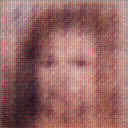
\includegraphics[width=150px]{500_fake_images/samples_5_431.png}%
\caption{A Man With A Beard Wearing A Tie}%
\end{figure}

%
\end{document}